%%%%%%%%%%%%%%%%%%%%%%%%%%%%%%%%%%%%%%%%%%%%%%%%%%%%%%%%%%%%%%%%%
%%%  The truth is out there and also in Twitter: analyzing Events via Name Entity Extraction %%%
%%%%%%%%%%%%%%%%%%%%%%%%%%%%%%%%%%%%%%%%%%%%%%%%%%%%%%%%%%%%%%%%%

\documentclass{sig-alternate}

% Fix for copyright block height
\makeatletter
\def\@copyrightlength{2.5} % Increase this value to leave more space above copyright notice
\def\ftype@copyrightbox{8}
\def\@copyrightspace{
\@float{copyrightbox}[b]
\begin{center}
\setlength{\unitlength}{1pc}
\begin{picture}(20,\@copyrightlength)
\put(0,-0.95){\crnotice{\@toappear}}
\end{picture}
\end{center}
\end@float}
\makeatother

\newcommand{\superscript}[1]{\ensuremath{^{\textrm{#1}}}}

\usepackage[hyphens]{url}
\usepackage{textcomp}
\usepackage{color}
\usepackage{listings}
\usepackage{multirow}
\usepackage{mathtools}
\usepackage{graphicx}
\usepackage{fancyvrb}
\usepackage{amsmath}
\usepackage{graphicx}
\usepackage[font=small,labelfont=bf]{caption}
\setcounter{MaxMatrixCols}{20}
\usepackage{pbox}

% listing styles
\lstset{numbers=left, numberstyle=\tiny,basicstyle=\ttfamily\scriptsize, tabsize=2, keywordstyle=\underbar, stringstyle=\small, backgroundcolor=\color[gray]{0.94}, framexleftmargin=2pt}
\lstdefinestyle{rdfa}{numberblanklines=true, morekeywords={}}

% Turtle box
\definecolor{olivegreen}{rgb}{0.2,0.8,0.5}
\definecolor{grey}{rgb}{0.5,0.5,0.5}
\lstdefinelanguage{ttl}{
sensitive=true,
morecomment=[l][\color{grey}]{@},
morecomment=[l][\color{olivegreen}]{\#},
morestring=[b][\color{blue}]\",
keywordstyle=\color{cyan},
morekeywords={version,owl,rdf,rdfs,xml,xsd,dbpedia,dbo,str,sso,scms,fr,ld}
}
\lstset{
        basicstyle=\ttfamily\scriptsize,
        upquote=true,
        showspaces=false,
        showstringspaces=false,
        showtabs=false,
        tabsize=2,
        frame=none,
        breaklines,
        numbers=none,
        framexleftmargin=2mm,
        xleftmargin=2mm,
}

\newcommand{\hilight}[1]{\colorbox{yellow}{#1}}
\newcommand{\todo}[1]{\colorbox{red}{#1}}

%\permission{Copyright is held by the International World Wide Web Conference Committee (IW3C2). IW3C2 reserves the right to provide a hyperlink to the author's site if the Material is used in electronic media.}
%\conferenceinfo{WWW'14 Companion,}{April 7--11, 2014, Seoul, Korea.}
%\copyrightetc{ACM \the\acmcopyr}
%\crdata{978-1-4503-2745-9/14/04.\\
%http://dx.doi.org/10.1145/2567948.2579326}
%\\Include the http://DOI string/url which is specific for your submission and included in the ACM rightsreview confirmation email upon completing your IW3C2 form}

\clubpenalty=10000
\widowpenalty = 10000

%%%%%%%%%%%%%%%%%%%%%%%%%%%%%%%
%%%  Beginning of document  %%%
%%%%%%%%%%%%%%%%%%%%%%%%%%%%%%%

\begin{document}

%\title{Named Entities for Analyzing Events in Twitter Stream}
\title{The Truth is out there and also in Twitter: \\ Analyzing Events via Name Entity Extraction}

\numberofauthors{5}
\author{
\alignauthor Jos\'e Luis Redondo Garc\'ia\\
	\affaddr{EURECOM}\\
	\affaddr{Biot, France}\\
	\email{redondo@eurecom.fr}
\alignauthor Giuseppe Rizzo\\
	\affaddr{EURECOM}\\
	\affaddr{Biot, France}\\
	\email{giuseppe.rizzo@eurecom.fr}
\and
\alignauthor Laurens De Vocht\\
    \affaddr{Ghent University - iMinds}\\
    \affaddr{Ghent, Belgium}\\
    \email{laurens.devocht@ugent.be}
\alignauthor Rapha\"el Troncy\\
	\affaddr{EURECOM}\\
	\affaddr{Biot, France}\\
	\email{raphael.troncy@eurecom.fr}	\\
}

\maketitle

%%%%%%%%%%%%%%%%%%
%%%  Abstract  %%%
%%%%%%%%%%%%%%%%%%

\begin{abstract}

Social platforms open a window to what is happening in the world in near real-time: microposts are constantly shared by people to report their experiences and feelings related to any type of events. Such an information can be collected and analyzed in order to get extra insights about what is happening out there regarding a particular event or story. However, the volume of information is very high and it is often difficult to extract such stories from a live social media stream. In this paper, we present a general framework to automatically mine social streams to provide journalists a set of headlines and complementary information that summarize the most important topics for a number of time-slots (time intervals) of interest. We describe an approach that collects fresh status from Twitter, groups them in time intervals and further analyzed them through deduplication, name entity extraction,  clusterization, and popularity reranking techniques. The final output is an temporarily ordered list of topics that aim to provide a summary of the most relevant insights about the studied event. 

\end{abstract}

% A category with the (minimum) three required fields
\category{H.3}{Information Storage and Retrieval}{Content Analysis and Indexing}

\keywords{Topic Generation, Name Entity Extraction, Storyboard Creation}

%%%%%%%%%%%%%%%%%%%%%%
%%%  Introduction  %%%
%%%%%%%%%%%%%%%%%%%%%%

\section{Introduction}
\label{sec:introduction}
The amount of videos shared on the Web is constantly increasing. We advocate the adoption of the Linked Media principles, where video segments are annotated with structured information and linked to other video segments. A new generation of innovative video services intend to use those semantic descriptions and media fragments for providing the users a novel experience where television content and web information are seamlessly interconnected.

The annotation problem has been traditionally addressed by applying multimedia analysis techniques \cite{ballan2011event}, but extracting semantic information from a video is still a challenging task. One possible approach consist in using Named Entity Recognition (NER) over the textual information attached to particular video fragment. Those techniques are an essential component within the Information Extraction field that focus on: identifying atomic information units in texts, named entities; classifying entities into predefined categories (also called context types) and linking to real world objects using web identifiers (Named Entity Disambiguation). A growing number of APIs provide such a service, like AlchemyAPI\footnote{\fontsize{8pt}{1em}\selectfont \url{http://www.alchemyapi.com/}} or DBpedia Spotlight\footnote{\fontsize{8pt}{1em}\selectfont \url{http://spotlight.dbpedia.org/}}. If the textual information attached to a video contains temporal references (e.g. subtitles), it is possible to align the entities with the time when they appear in the video. Katsiouli et al.~\cite{katsiouli2007} have demonstrated that applying named entity recognition techniques in combination with domain ontologies on video subtitles can produce good results for video classification.


A screencast showing an example of these functionalities is published at \url{http://youtu.be/jIMdnwMoWnk} while the system is publicly available at \url{http://mediafinder.eurecom.fr/story/elezioni2013}.


The massive amount and steady increase of heterogeneous data shared on social platforms has attracted the interest of different research communities. Microposts such as status updates or tweets enable people to share their activities, feelings, emotions and conversations, opening a window to the world in real-time. Making sense out this amount of data is an extremely challenging task due to its heterogeneity (media items mixed with textual data) and dynamics making often short-lived phenomena. A growing number of commercial tools and academic research approaches try to partially collect and analyze this data in order to make sense of it. Capturing life moments and building narratives using social platforms is, for example, the goal of Storify\footnote{\url{http://storify.com}} where the creators aim to investigate the interaction between event stories and the role of social networks that tell them: \textit{(i)}~sorting and organizing the items of an experience similar to the elements of a story, \textit{(ii)}~communicating and discussing strategies on how to guide a user towards an intended experience. The overall storytelling creation is supervised by the user who composes a story based on streams of news coming through social platforms such as Twitter and YouTube. Generating the big picture from these streams is also the objective of Storyful\footnote{\url{http://storyful.com}}. This application enables the user to navigate through the story created by other users or to create his own, aggregating content from different social platforms. While these two approaches position the role of a social platform as a container of fresh and breaking news items, they are leveraging on the user interaction that defines the summary creation as a supervised task. A disruptive innovation has been recently revealed by Mahaya\footnote{\url{http://mahaya.co}} which proposes an automatic crowd storyfication of the 12/12/12 concert\footnote{\url{http://121212.mahaya.co}}. In this example, the highlights of the concert corresponding to social media spikes when performers appeared are emphasized with images collected from Instagram, and microposts collected from Twitter. Inspired by the idea of automatic summarization through visual galleries, we focus more on the automatic sorting and clustering of media items for topic visualization. In~\cite{Rizzo2012}, we proposed a generic media collector for retrieving media items that illustrate daily life moments shared on social platforms. In particular, we proposed a common schema in order to align the search results of numerous social platforms. This demonstration extends~\cite{Milicic2013}, adding to the codebase, the temporal feature to the cluster operations.

~\cite{Aiello}

~\cite{Schifferes}

%%%%%%%%%%%%%%%%%%
%%%  Approach  %%%
%%%%%%%%%%%%%%%%%%

\section{Approach}

We describe the steps applied over the a stream of microposts coming from Twitter in order to select and highlight the main topics about high coverage events. To reconstruct those different topics that better illustrate a particular fact being discussed in Twitter, we apply different techniques that go from collection and normalization of the tweets related with the event to name entity extraction an clustering, in order to infer which are the most relevant aspects that the crow has been commenting about.

The complete processing workflow takes as input a set of keywords which evoke the event to be tracked, a list of user accounts to monitorize, and the start and end times for which that particular event is considered. Of course we assume that the studied event has a minimal presence and coverage on the Web to ensure that there are a sufficient Twitter activity that illustrates it and allows to reconstruct what has happened in there. 

The output of the algorithm is a temporally ordered list of relevant topics for the given event, which in turn contain a set of more detailed attributes that are further explained in Section~\ref{sec:expansion} Our hypothesis states that this set of event topics provides a set of valid headlines and complementary information that summarize the most important facts behind that particular story. 

\subsection{Tweet Collection}

The tweets used as input for this approach are extracted by using the Twitter streaming API \footnote{\fontsize{8pt}{1em}\selectfont \url{https://dev.twitter.com/docs/streaming-apis}} from a set of predefined list of keywords and user accounts. For making easier this task we have used an already existing tool available in here\footnote{\fontsize{8pt}{1em}\selectfont \url{https://github.com/socialsensor/twitter-dataset-collector}}. The tweets obtained are represented following a JSON schema that has been simplified for reduce the complexity the subsequent steps of the analysis. Also, a near-deduplication process is launched in order to group tweets with highly similar textual content: as many users copy the content of other status without using the retweet/reply option or explicitly mention the original tweet, we programmatically detect those tweets and consider them together in the following steps.

\subsection{Temporal groping and Named Entity Extraction}

Before passing to the next step, we have sliced the entire tracking time period into smaller slots where the different tweets are aligned to. This time dimension is one of the key aspect of an event, but it is strongly depending on the nature of the event and the consumption needs of the person that is tracking the event. Due to this particular parameters playing a role in the time slot's duration decision, we have decided to simply assume this number as a external parameter that has to be specified in advance for fitting as well as possible to the particular scenario. Finally we have discarded the microposts published outside the boundaries of the total interval, obtaining a list of tweets group ordered by time which will be analyzed in order to discover important facts about the studied event.

For each status retrieved, we perform named-entity recognition over the corresponding tweet using the NERD framework~\cite{Rizzo2012}. In our experiment the language of the tweets is restricted to English but NERD supports other languages. The output of this phase is a list of tweets with its corresponding entities annotated using the NERD ontology\footnote{\fontsize{8pt}{1em}\selectfont \url{http://nerd.eurecom.fr/ontology/nerd-v0.5.n3}} and a relevance score obtained from the extractors which have been used. 

\subsection{Entity Clustering }
\label{sec:expansion}

Once the Named Entities have been obtained, a first clustering operation is performed over the tweets of every time-slot for determining which are the most frequent entities in them. First, we iterate over all the available disambiguation URLs for finding how many different entities are available, and then for each detected URL we attached the list of tweets that mention it. Note that the same tweet can appear under different entity clusters since more than one entity could have been spotted in its text. At a first glance, those entities constitute a primitive way of generating topics about the studied event, and the cardinality of the number of tweets associated to them gives an idea about their importance. Figure~\ref{fig:EntityCluster} shows in more detail this operation: a set of different topics corresponding to named entities have been extracted and ordered according tho the number of tweets in which they appear.

\begin{figure}[h!]
\centering
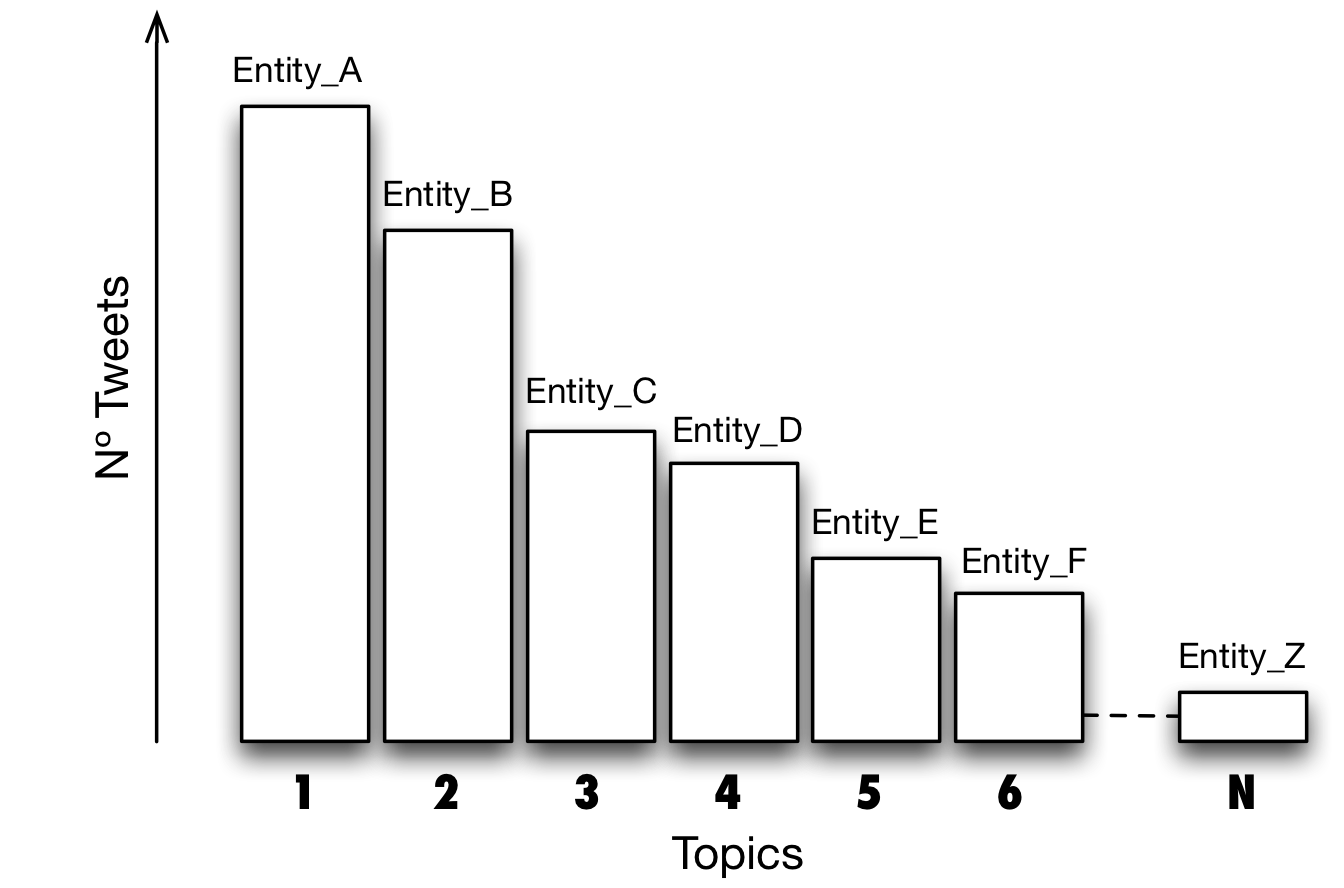
\includegraphics[width=0.4\textwidth]{figure/EntityCluster.png}
\caption{Clustering Named Entities according to their frequency in the Tweets corpora.}
\label{fig:EntityCluster}
\end{figure}

\subsection{Hierarchical clustering}

Next step consist of executing a method of cluster analysis which builds a hierarchy of groups were certain elements are merged on t where one or more groups of tweets are merged together because they present similar characteristics. In particular this particular implementation follows an agglomerative "bottom up" approach: each pair of observations witch similar characteristics of clusters are merged together. In order to decide which clusters should be combined, we have defined a measure of similarity between different sets of observations. In particular, we determine which clusters share a significant amount of tweets, groping them together when is the case. We iterate over all the possible pairs of clusters available in the time slot, including the ones that are created during the process. The process stops when no more candidate pairs are found to be merged. 

\begin{equation}
\begin{split}
\forall A, B \in Topic_{Entity}, Sim (A,B) =\frac{\left | tweets(A) \cup  tweets(b) \right |}{\left | tweets(A) \cap  tweets(b) \right |} \\
Delete(A, B) \wedge Create(C) \Leftrightarrow  Sim (A,B) > Threshold \\
C= \text{tweets(A)} \cup \text{tweets(B)}
\end{split}
\end{equation}


In Figure~\ref{fig:Hierarchical_Cluster} we observe how the clusters corresponding to \textit{Entity\_C} and \textit{Entity\_D} are combined together since the last contains a high percentage of the tweets from the first. The result is a new cluster labelled with both original entities that contains the union of the tweets coming from them.

\begin{figure}[h!]
\centering
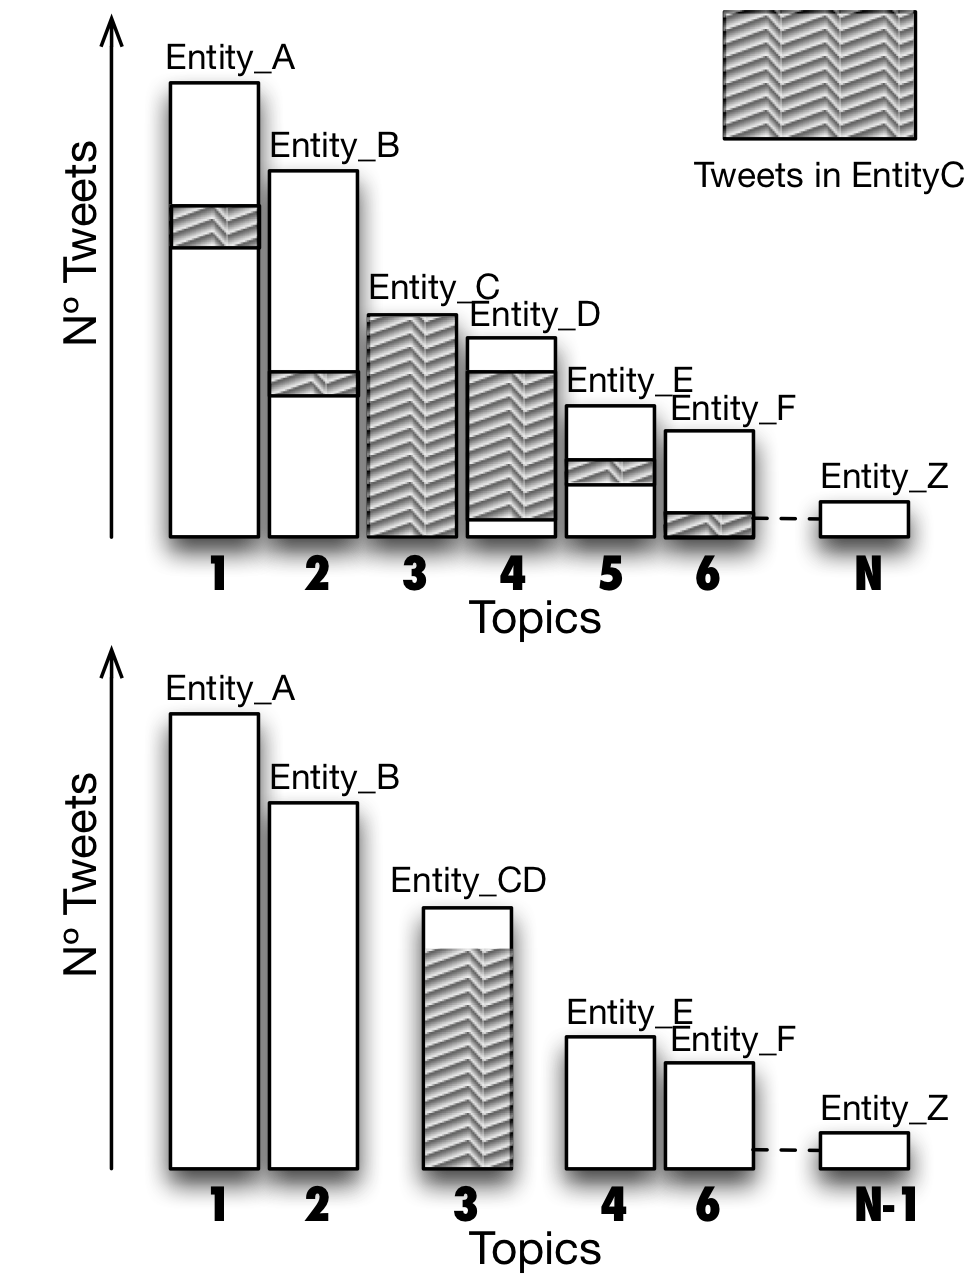
\includegraphics[width=0.4\textwidth]{figure/Hierarchical_Cluster.png}
\caption{Applying hierarchical clustering over entity clusters according to tweets coexistence.}
\label{fig:Hierarchical_Cluster}
\end{figure}

\subsection{Inverse Frequency Ranking}

The topics obtained so far have been ordered by taking into account the number of tweets where the corresponding entities have been found. However, the fact that an entity has an higher frequency in the entire corpora does not mean it is more relevant for that certain period of time. In many cases, the most repeated words are indeed the more general ones and therefore are not the most suitable for characterizing the smaller stories that compounds the entire event. In order to take in consideration this phenomena, we calculate an inverse topic frequency in order to reflect how discriminating is a certain cluster inside the context of the entire corpus. 
Consequently, the final score increases proportionally to the number of times an entity appears in the set of tweets, but is offset by the frequency of the entity in the rest of clusters, which helps to control for the fact that some entities are more common than others. The implemented logic is summarized in the following equation:

\begin{equation}
\text{idf}(e, Slot) =\frac{N_{topics}}{\left | x\in Topics: \left | \text{tweets}(e)\cap \text{tweets}(x) < T_{20}\right |\right |}
\end{equation}

For every topic notated as $e$, this formula generates a score that increases with the total number of topics inside the time-slot and decreases with the number of other topics that contains a significant amount of tweets belonging to $e$. As displayed in Figure~\ref{fig:TF-IDF} the tweets in the cluster \textit{Entity\_D} are less spread all over the rest of topics in the time-slot that the ones from \textit{Entity\_C} that can be found in a signgicant number in \textit{Entity\_A},  \textit{Entity\_B} or  \textit{Entity\_E}. In consequence, \textit{Entity\_D} can be promoted against \textit{Entity\_C} for reflecting its higher discriminate rate.

\begin{figure}[h!]
\centering
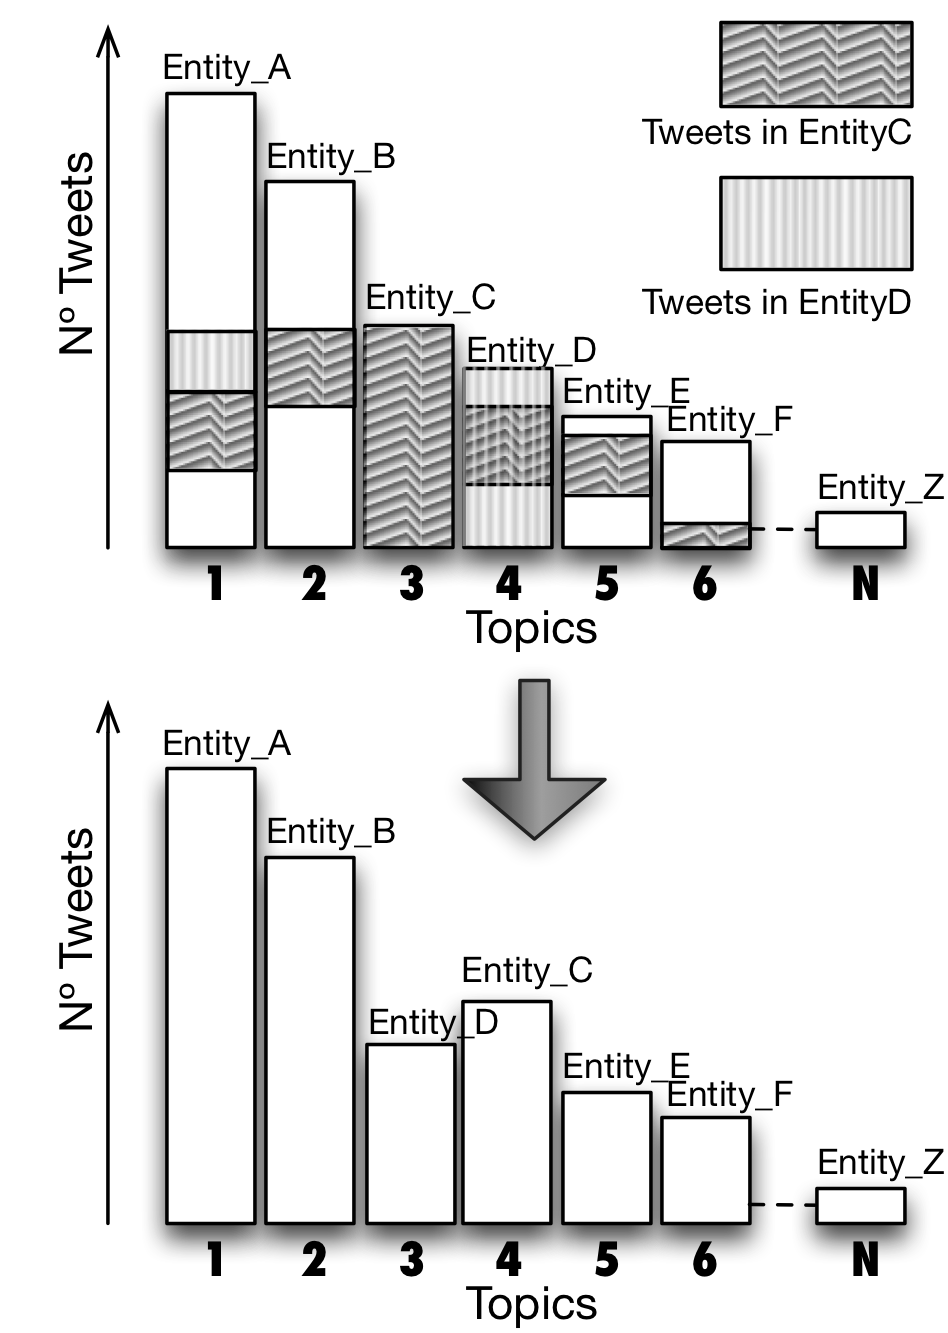
\includegraphics[width=0.4\textwidth]{figure/TF-IDF.png}
\caption{Ranking entity clusters according to inverse frequency in the rest of topics.}
\label{fig:TF-IDF}
\end{figure}

\subsection{Tracking Topics}

The importance of the temporal dimension in social media monitor tasks is crucial: we can not properly understand what is happening in the present without taking a look at the past. This aspect becomes even more relevant when trying to make sense out the noisy data from social networks, where the more clues we have about the present items the better results we get. It is surprising the same exact data collected for a particular time-slot can be differently interpreted depending on previous analysis about the same facts. In order to deal with this phenomena our approach implements a logic that takes into account the previous states of the detected topics when ranking and filtering them. 

In particular, we take into account two different features: the variation in the topic's tweet frequency from the former state to the current one, and a vector of scores that keeps a record about the tendency of the topic during the last states and is updated after every iteration.

\begin{equation}
\begin{split}
V_{tendency} = \left \{ s_{1} , s_{2} , s_{3} ... s_{n} \right \} :s_{n} \in (0,\mathbb{R}), \\
\left | V_{tendency}  \right |=\left | \bigcup_{n}^{0} Topic_{Entity_N}  \right |
\end{split}
\end{equation}

The final score combines together both measures as follows in order to provide the notion of topic tracking:

\begin{equation}
Trac_{n}^{t} = \left | Topic_{N} \right | *\left ( 1+\frac{\left | Topic_{N}\right |  - \left | Topic_{N-1}\right | }{max \left ( \left | Topic_{N}\right | , \left | Topic_{N-1}\right |  \right ) } \right ) * s_{n}^{t}
\end{equation}

The $V_{tendency}$ vector is updated as follows from one iteration to the other:

\begin{equation}
s_{n}^{t} = s_{n}^{t-1} *\left ( 1+\frac{\left | Topic_{N}\right |  - \left | Topic_{N-1}\right | }{max \left ( \left | Topic_{N}\right | , \left | Topic_{N-1}\right |  \right ) } \right ) * \beta
\end{equation}
\begin{itemize}
  \item A new topic T as always an tendency score $s_{t}$ equal to 1(neutral value).
  \item By default, a tendency score $s_{t}$ is reduced in a certain rate $\beta$ from one state to the following.
  \item The tendency score $s_{t}$ decreases faster if the tendency is negative.
  \item The tendency score $s_{t}$ increases if the tendency in the last states has been positive enough.
\end{itemize}

In Figure~\ref{fig:Tracking} it is possible to see how the scores from time $t-1$ are combined together with the one calculated in $t$ for outputting a more accurate ranking about the importance of the topics detected.

\begin{figure}[h!]
\centering
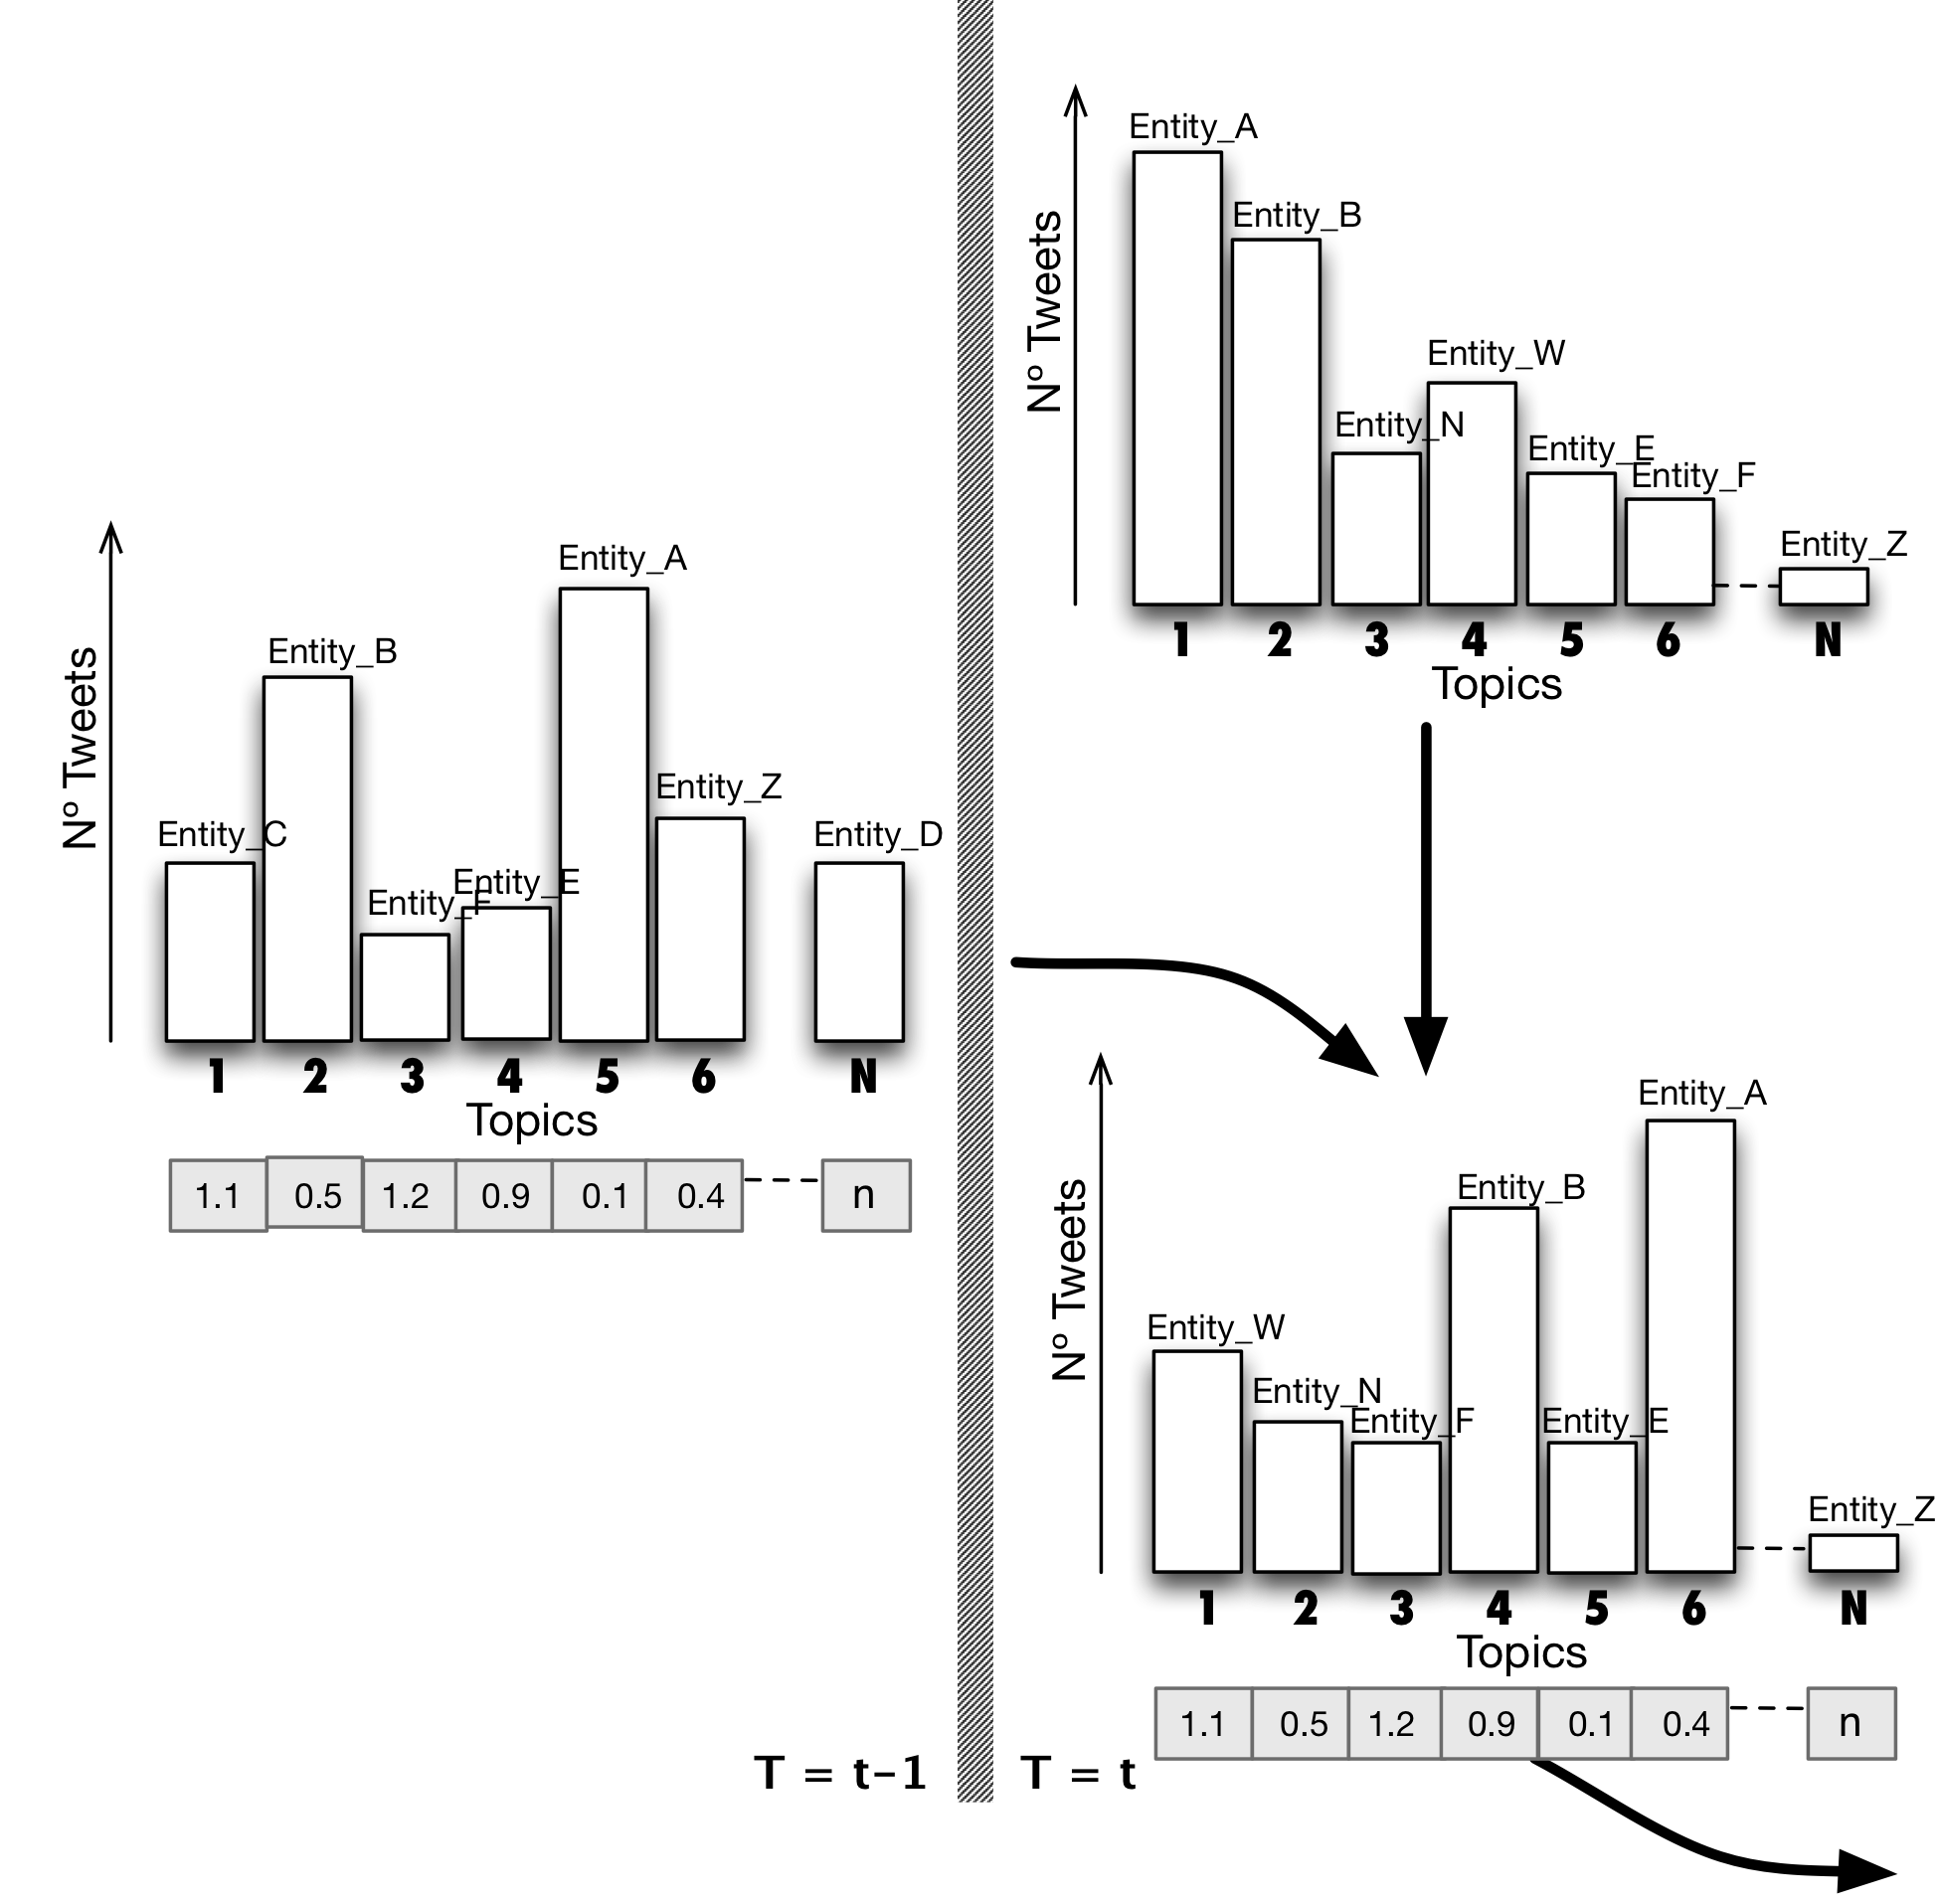
\includegraphics[width=0.5\textwidth]{figure/Tracking.png}
\caption{Using the evolution of previously calculated topics for reranking the present ones.}
\label{fig:Tracking}
\end{figure}

Even the topic relevance order is directly influenced by the scores from the last time-slot analysis and implicitly from the previous ones via the $V_{tendency}$ vector, the tracking logic could be further improved by explicitly considering more than one previous states and make more precise judges regarding the negative or positive slope of the tweet frequency curve. Another intrinsic issue of any tracking approach is the \textit{cold start} problem: when analyzing the first time-slot for a particular event, we have no indications about how first data collected looked like before. This problem can be alleviated by increasing the temporal window via an early start of the collection process.

The algorithms for ranking clusters and the ones for tracking their changes in time should be closely tied in order to maximize the quality of the final topics. The different behavior of events make some approaches more suitable than others for certain kinds of events, but the way the accuracy of a topic detection varies for a particular kind of event is a research question that will not be studied in this paper.


\subsection{Popularity Measures}
In this phase, the additional documents which have just been retrieved are now processed and analyzed in order to extend and re-rank the original set of entities and consequently get a better insight about the event. Since most of the resources retrieved are Web pages, HTML tags and other annotations are removed, keeping only the main textual information. This plain text is then analyzed by the NERD framework in order to extract more named entities.

POPULARITY of a tweet.


\subsection{Stadistics.}


\subsection{Tweet popularity.}


\subsection{Peak Detection}

In order to calculate the frequency of a particular resource within the entire corpora, we group the different appearances of the same instance and check their cardinality. This is not a trivial task since the same entity can appear under different text labels, contain typos or have different disambiguation URL's pointing to the same resource. We performed a centroid-based clustering operation over the instances of the entities. We considered the centroid of a cluster as the entity with the most frequent disambiguation URL's that also have the most repeated labels. As distance metric for comparing pairs of entities, we applied strict string similarity over the URL's, and in case of mismatch, the Jaro-Winkler string distance~\cite{winkler2006overview} over the labels. The output of this phase is a list of clusters containing different instances of the same entity.

Formula

Figure~\ref{fig:Peaks}.


\begin{figure}[h!]
\centering
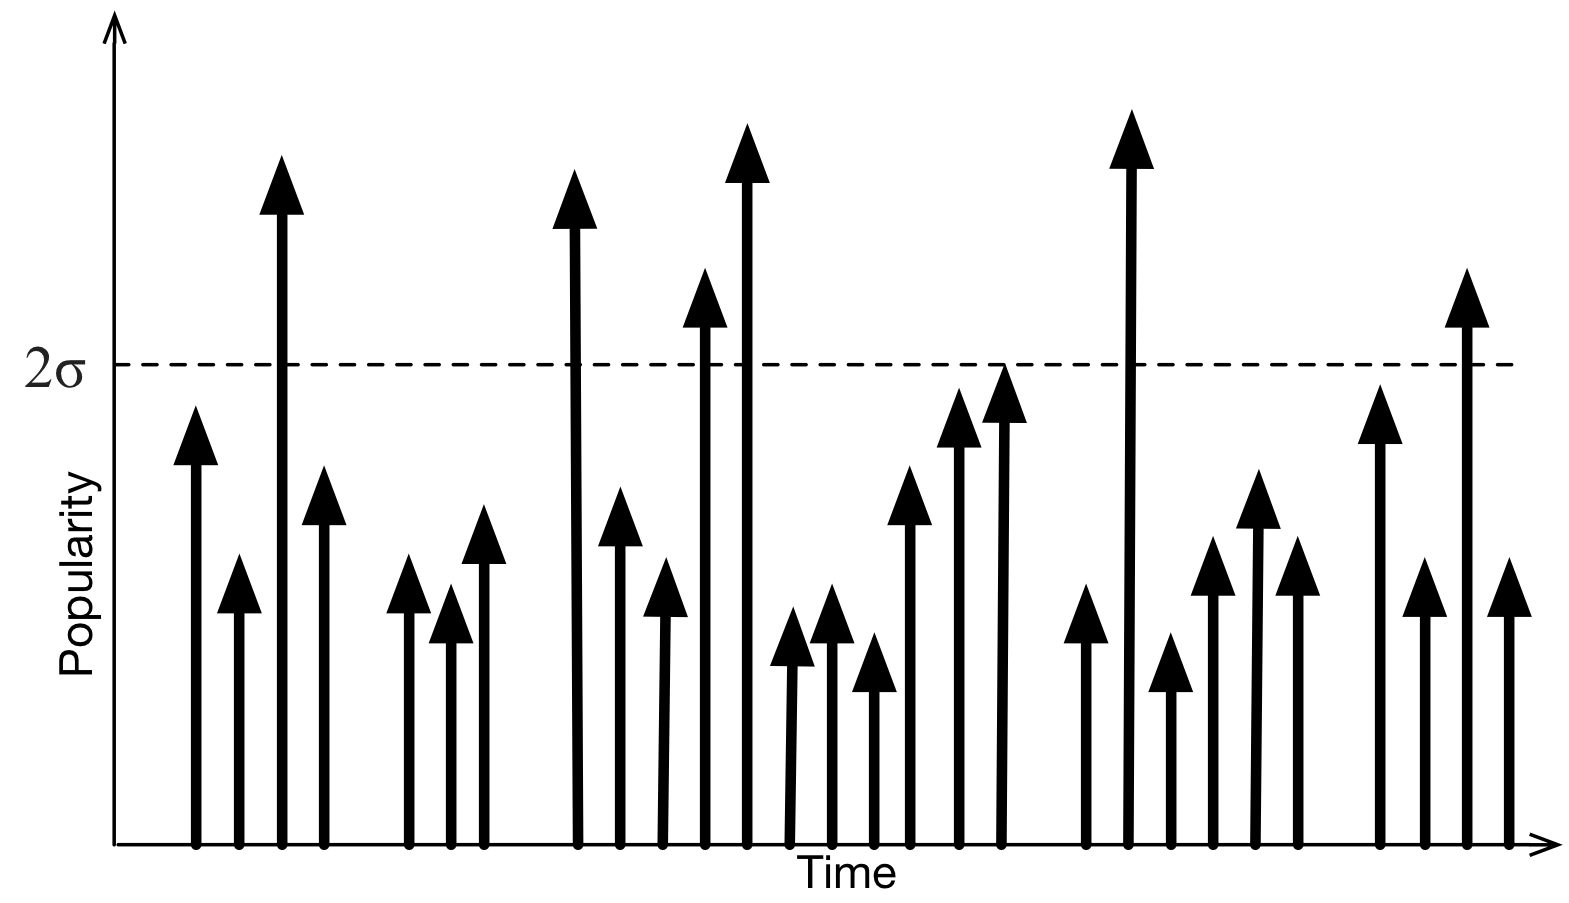
\includegraphics[width=0.4\textwidth]{figure/Peaks.png}
\caption{Detecting peaks inside a particular topic..}
\label{fig:Peaks}
\end{figure}


\subsection{Peak Tracking}
The final step of the expansion consists of ranking the different named entities obtained so far. To create this ordered list, we assigned a score to every entity according to the following features: relative frequency in the transcripts of the event video; relative frequency over the additional document; and average relevance according to the named entity extractors. The three dimensions are combined via a weighted sum where the frequency in the video subtitles has a bigger impact, followed by the frequency on the searched documents and the relevance from the extractors. The final output of the entity expansion operation is a list of entities together with their ranking score and the frequency in both the main video and in the collected documents retrieved from the search engine.

Formula
For ranking results and generate results (see next section)

Entities with a higher $relScore_{i}$ in the final classification are considered more representative for describing the context than the original entities. Furthermore, we observe that:
\begin{itemize}
  \item The bigger the sample size, and the better becomes the ranking. Entities appearing repeatedly in the additional documents will be promoted while those appearing rarely will be pushed back to the end of the list.
  \item Entities that originally have not been disambiguated can now have their corresponding URL if any of the similar instances appearing in the additional documents provide a link to a Web resource. The same occurs with incomplete or misspelled labels.
  \item Finally, some entities not spotted in the original transcripts but important in the context of the event are now included in the list of relevant items since they have been extracted from the collected documents.
\end{itemize}

FILTER ONLY WITH HIGH X BEFORE SERIALIZE
\subsection{Generating results}
\label{sec:results}

Once the set of context relevant entities has been expanded, we will use the knowledge from structured sources to reinforce the important entities and finding relevant predicates between them.

\subsubsection{main tweets}
In this step, the DPpedia path finding technique implemented in~\ref{sec:dbpedia_path} is applied over the set of entities obtained via entity expansion. Since this list is too broad, we need to establish in first place a division between what we consider the \textit{mainEntities}(entities whose relative scores fall under the higher 25\% of the relevance range), and the \textit{additionalEntities}(the rest of entities in $E_{Expansion}$).

\subsubsection{keywords}

\subsubsection{images}

\subsubsection{text}


- time/date in the format DD-MM-YY hh:mm, example: 26-02-14 10:15
(this is the beginning of the timeslot)
- topic title: Make sure the title doesn't contain newline or tab characters!
- tags: Comma-separated list of tags. 
- ids: Comma-separated list of tweet ids
- image URL (optional): A valid image URL. The URL should end with .jpg, .png or .gif.


In the future, we plan to use the frequency measures about predicates available in $F_{prop}$ in order to more precisely rank the named entities. By using the \textit{commonalities} function (\url{http://demo.everythingisconnected.be/commonalities?between=Res1&and=Res2&allowed=property}) over the set of $mainEntities$ inside $Entities_{Extension + DBpedia}$ and for the properties with highest $F_{prop}$, we obtain the set of entities directly related with the original ones through the top predicates. Once more, the most frequent entities in Commonalities could promote the already existing entities in $Entities_{Extension + DBpedia}$.

%%%%%%%%%%%%%%%%%%%%%%%%%%%%%%%%%%%
%%%  Use Case: USA Elections 2012  %%%
%%%%%%%%%%%%%%%%%%%%%%%%%%%%%%%%%%%

\section{Use Case: Snowden Assylum}
We have applied this method over a real scenario corresponding to the news video \url{http://www.bbc.co.uk/news/world-europe-23339199}, from the BBC News Europe Web site. The main story behind this media content is the request of asylum made by Edward Snowden to the Russian government. In an airport in Moscow, he publicly express his desire to obtain political help while he can find a safe way to reach the Latin American countries that offer a safe harbor. The time period for which this particular event is relevant goes from 2013-07-06 to 2013-07-17.

\subsection{Named Entity Extraction}
In a first step, Name Entity Extraction techniques are applied over the video transcript using NERD. We show below the list of entities directly extracted via this procedure, which brings a first approximation to the context of the news media item.
\begin{table}[tbp]
  \resizebox{8cm}{!} {
\begin{tabular}{ c | c | c | c | c }
  \hline
 Label & Relevance & Sentiment & Type & URI  \\ \hline
Russia & 0.809216 & Mixed & Location & DBpedia:Russia \\
Edward Snowden & 0.717369 & Mixed & Person & DBpedia:/Edward\_Snowden \\
South America & 0.56586 & Mixed & Location & DBpedia:South\_America \\
president Putin & 0.459811 & positive & Person & DBpedia:Vladimir\_Putin \\
president & 0.401138 & negative & JobTitle & DBpedia:President \\
Moscow & 0.352101 & Mixed & City & DBpedia:Moscow \\
CIA & 0.334887 & neutral & Organization & DBpedia:CIA \\
Bolivia & 0.324607 & neutral & Location & DBpedia:Bolivia \\
Obama & 0.321901 & negative & Person & DBpedia:Barack\_Obama \\
  \hline
\end {tabular}
  }
\caption{Raw result from Named Entity Extraction with NERD}
\end{table}

\subsection{Named Entity Expansion}
In a second step, the original set of entities is expanded as described in Section~\ref{sec:expansion}. The query generated for retrieving additional documents has the text ``Edward Snowden asylum Russia'', and is bounded to the period from 2013-07-06 to 2013-07-28. After analyzing the additional documents retrieved by the search engine, the instances are re-ranked according to their global frequency.

The final result after the expansion operation is a bigger list of entities (more than 100). In some cases, the previously spotted entities (like \textit{Extradition}) have been promoted in the hierarchy while others (like \textit{Right\_of\_asylum\\}) have been discovered in the new documents. For this use case, we have taken only a fixed number of top entities ($mainEntities = 15$). Those entities will be used as input to the third step of context refinement.

STAtistics about number of entities


\subsection{Final result}
Given the set of $mainEntities$ obtained from the Named Entity Expansion operation, we study how close two graph nodes $e_{i}$, and $e_{i}$ are connected according to the normalized average length of all the intermediate paths between them in DBPedia. The results are expressed in the form of an adjacency matrix, which allows to visually analyze the connections between pairs of entities inside $mainEntities$.

\begin{table}[tbp]
  \resizebox{8.5cm}{!} {
\begin{tabular}{  c | c | c | c }
  \hline
    \multicolumn{2}{c|}{Nodes} &
    \multicolumn{2}{c}{Properties} \\
  \hline
  URL & Frequence & URL & Frequence \\ \hline
DBpedia:Wilmington,\_North\_Carolina & 14 & http://dbpedia.org/ontology/country & 44 \\
DBpedia:United\_States & 38 & http://dbpedia.org/ontology/birthPlace & 64 \\
DBpedia:Russia & 12 & http://purl.org/dc/terms/spatial & 42 \\
DBpedia:conference/AIPR/2008 & 11 & http://dbpedia.org/ontology/almaMater & 26 \\
DBpedia:Washington,\_D.C. & 10 & http://dbpedia.org/ontology/location & 21 \\
DBpedia:Igor\_Panarin & 8 & http://dbpedia.org/ontology/profession & 20 \\
DBpedia:Chap\_Petersen & 8 & http://dbpedia.org/ontology/nationality & 14 \\
DBpedia:North\_Carolina & 8 & http://dbpedia.org/property/leaderTitle & 14 \\
DBpedia:Independent\_(politician) & 8 & http://dbpedia.org/ontology/occupation & 14 \\
  \hline
\end{tabular}
  }
\caption{Top middle nodes and properties inside DBpedia paths}
\label{table:frequentNodesProp}
\end{table}

The $Conectivity$ scores are combined together with the frequency of intermediate nodes in the paths ($F_{inPaths}$) and the former relevance indexes from the entity extension phase ($Rel_{extension}$) for obtaining a new ranked list of entities that intends to better represent the context of the news event.

\subsection{Evaluation}
\label{sec:evaluation}

We have evaluated the result obtained by our approach against a set of entities provided by an expert. We plan to extend this evaluation to a larger corpora and include a more exhaustive evaluation in future work. We start from the list of entities provided by the expert, together with some insights about the relevance of the concept inside the scope of the video:

We first evaluate the set of entities spotted by the expert against traditional Named Entity Extraction results from NERD. About precision and recall, 3 entities have been spotted out of the 7 while in total 12 were proposed as candidate results. The lawyer of the case, Anatoly Kucherena, is never mentioned in the subtitles, so it has not been detected. Even if the word airport is present in the subtitles, we are not sure which one is relevant given that there are two airport in Moscow.

Finally, we compare the expert's feedback against the final DBpedia $E_{Expansion + DBpedia}$ ranked set of entities. There are no differences for the spotted \textit{MainEntities}. However, we observe that other improvements have been achieved concerning the ranking order inside \textit{MainEntities}. For example, the entity ``Sheremetyevo'' is now scored higher, which makes sense from the event's perspective since it is the most specific location where the action takes place. Some other relevant entities include the prime Minister of Russia, Igor Shuvalov, which was not detected via entity expansion. They have not been included in the set of results but we will study this possibility for future developments. Also, the adjacency matrix opens room for many other context analysis like topic clustering, which could help to give further insights about an event.

"The official evaluation results of our method in the Data Challenge are included in \cite{snow2014dc}."

- subjective evaluation (based on human assessment) of selected topics;
- automatically computed diversity measures (e.g. cosine similarity between topics)
- present sample topics produced by your method (including images)
- in case your method uses parameters explain how you selected them, and how they affected results
- basic statistics of produced topics (e.g. most frequent topic tags)
- any other idea is welcome - try to be creative!


%%%%%%%%%%%%%%%%%%%%%
%%%  Conclusions  %%%
%%%%%%%%%%%%%%%%%%%%%

\section{Conclusions}
We presented an approach for context-aware annotating news events, designed to precisely harvest program descriptions starting from named entities recognized in TV video transcripts. Because the entities initially spotted are typically insufficient for covering the broader range of concepts that best describe a particular news clip, we expanded this set by analyzing additional textual documents about the same event.

The flat ranked list of concepts is afterward completed with cues about their connectivity obtained by analyzing the DBpedia paths that exist between them. In particular, we promoted entities which are better interlinked inside the context and with higher frequency in the nodes of the generated DBpedia paths. Finally, we identify the important predicates linking those entities. This leads to a more accurate re-ranking of the entities belonging to this news event.

The preliminary results indicate that we can successfully expand the initial set of recognized entities with more relevant concepts not detected by pure named entity recognition approaches. Exploring DBpedia paths along the named entities occurring in news media leads to a more accurate ranking of important concepts and even if it does not necessary introduce any new top item, it brings forward more related entities with additional information about the broader context of an event.

- Something as simple as doing a first text cleaning/reprocessing of the tweets would have boosted (imho) the final results: for example, grouping tweets that have -almost- the same text (some people just c\&p other tweets and add some extra punctuation sign or small expression) will significantly improve the subsequent clustering operations.
- Further analyze the temporal dimension: even we are dividing the event period into time slots, it is crucial to properly track how the clusters change over the time, in order to discard noisy data from previous events and emphasize what is really new. Indeed there is a sort of cold start problem with first topics in the interval, since we don't know what happened before.
- Use the original JSON format as it comes from the Twitter Stream API. This is not entirely our fault because at the beginning the organizers gave us a different reduced schema and we prepared our subsequent tools for working over it� but Twitter originally provides a more much rich metadata where for example they already include what they call "entities" (hashtags and keywords). 


%ACKNOWLEDGMENTS are optional
\section*{Acknowledgments}
This research has been partially funded by the European Union's 7th Framework Programme via the project LinkedTV (GA 287911) and Ghent University.
%iMinds (Interdisciplinary institute for Technology) a research institute founded by the Flemish Government,
%the Institute for the Promotion of Innovation by Science and Technology in Flanders (IWT), the Fund for Scientific Research-Flanders (FWO-Flanders),

REFERENCE MEDIAFINDER PAPER.
ReFERENCE MEDIA COLLECTOR??

\bibliographystyle{abbrv}
\bibliography{snow_challenge}

\end{document} 